
\chapter{Modelli atomici}
\label{chap:modAtom}

\section{Teoria atomica di Dalton}
\label{sec:teoriaatomdidalton}
\begin{tteor}
  Atomi costituiti da una nuola di carica positiva neutralizzata da elettroni in un modello a panettone
\end{tteor}
\begin{figure}[ht!]
  \centering
  % colors
\definecolor{mylightred}{RGB}{255,210,210}
\definecolor{myred}{RGB}{200,100,100}
\definecolor{mydarkred}{RGB}{140,40,40}
\definecolor{mylightblue}{RGB}{220,228,255}
\definecolor{myblue}{RGB}{183,191,229}
\definecolor{mydarkblue}{RGB}{50,70,190}

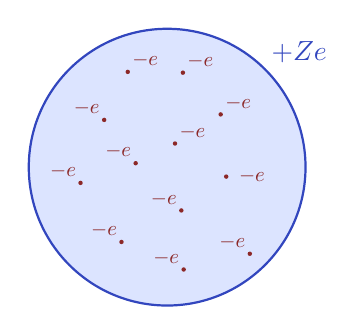
\begin{tikzpicture}[scale=1]
    \coordinate (O)  at (0,0);
  \draw[mylightblue,fill] (O) circle (50pt);
  \draw[mydarkblue,thick] (O) circle (50pt) node[above right=34pt] {$+Ze$};
  \fill[radius=0.8pt,mydarkred]
    ( 0.20, 1.20)  circle node[above right=-1pt,scale=0.75] {$-e$}
    ( 0.10, 0.30)  circle node[above right=-1pt,scale=0.75] {$-e$}
    ( 0.68, 0.67)  circle node[above right=-1pt,scale=0.75] {$-e$}
    ( 1.05,-1.10)  circle node[above left =-1pt,scale=0.75] {$-e$}
    ( 0.75,-0.12)  circle node[      right= 2pt,scale=0.75] {$-e$}
    ( 0.21,-1.30)  circle node[above left =-1pt,scale=0.75] {$-e$}
    ( 0.18,-0.55)  circle node[above left =-1pt,scale=0.75] {$-e$}
    (-0.80, 0.60)  circle node[above left =-1pt,scale=0.75] {$-e$}
    (-0.50, 1.21)  circle node[above right=-1pt,scale=0.75] {$-e$}
    (-0.40, 0.05)  circle node[above left =-1pt,scale=0.75] {$-e$}
    (-0.58,-0.95)  circle node[above left =-1pt,scale=0.75] {$-e$}
    (-1.10,-0.20)  circle node[above left =-1pt,scale=0.75] {$-e$};
\end{tikzpicture}

  \caption{Modello atomico di Dalton}
  \label{fig:modatomDalton}
\end{figure}
Sostanzialmente Dalton suppose che l'atomo fosse un modello sferico in cui la carica positiva circondava
le carriche necative che erano presenti al suo interno esattamente come le uvette o i canditi
all'interno di un panettno o di un Plum pudding, ovviamente questo modello agli occhi dei dati odierni
fa un po' sorridere ma è già un punto di inizio. Non si parla ancora di orbite, di neutroni o di della
composizione del nucleo.

\section{Esperimento e modello atomico di Rutherford}
\label{sec:rutherford}

\begin{tteor}
  Atomo nucleare costituito da un nucleo formato da protoni e neutroni circondando da un numero di
  elettroni pari ai protoni.
\end{tteor}
\begin{figure}[ht!]
  \centering
  % colors
\definecolor{mylightred}{RGB}{255,210,210}
\definecolor{myred}{RGB}{200,100,100}
\definecolor{mydarkred}{RGB}{140,40,40}
\definecolor{mylightblue}{RGB}{220,228,255}
\definecolor{myblue}{RGB}{183,191,229}
\definecolor{mydarkblue}{RGB}{50,70,190}

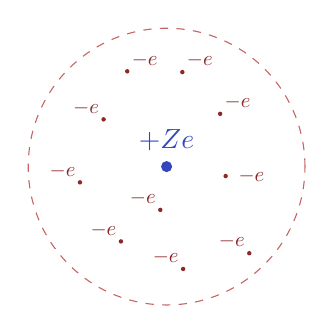
\begin{tikzpicture}
 \coordinate (O)  at (0,0);
  \draw[myred,dashed]            (O) circle (50pt);
  \fill[radius=2.0pt,mydarkblue] (O) circle node[above=2pt] {$+Ze$};
  \fill[radius=0.8pt,mydarkred]
    ( 0.20, 1.20)  circle node[above right=-1pt,scale=0.75] {$-e$}
    ( 0.68, 0.67)  circle node[above right=-1pt,scale=0.75] {$-e$}
    ( 1.05,-1.10)  circle node[above left =-1pt,scale=0.75] {$-e$}
    ( 0.75,-0.12)  circle node[      right= 2pt,scale=0.75] {$-e$}
    ( 0.21,-1.30)  circle node[above left =-1pt,scale=0.75] {$-e$}
    (-0.80, 0.60)  circle node[above left =-1pt,scale=0.75] {$-e$}
    (-0.50, 1.21)  circle node[above right=-1pt,scale=0.75] {$-e$}
    (-0.08,-0.55)  circle node[above left =-1pt,scale=0.75] {$-e$}
    (-0.58,-0.95)  circle node[above left =-1pt,scale=0.75] {$-e$}
    (-1.10,-0.20)  circle node[above left =-1pt,scale=0.75] {$-e$};

\end{tikzpicture}
  \caption{Modello atomico di Rutherford}
  \label{fig:modatomRutherford}
\end{figure}

\subsection{Esperimento di Rutherford}
\label{sec:esperimentodiruth}
L'esperimento di Rutherford sulla deviazione di particelle $\alpha$ (\ce{He2+}) da parte di sottili lamine d'oro (600nm). Lampi di luce segnalano dove le particelle alfa hanno colpito lo schermo.
\begin{figure}[ht!]
  \centering
  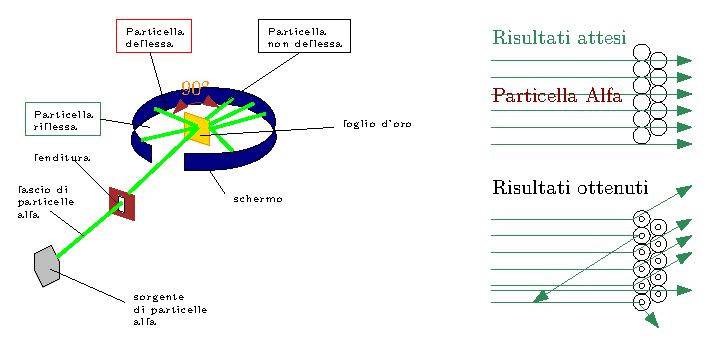
\includegraphics{./img/espRuth.eps}
  \caption{Illustrazione dell'esperimento di Rutherford}
  \label{fig:espruther}
\end{figure}\\
Una particella in movimento ed un elettricamente carica perde incessantemente energia, questo vale
anche per l'elettrone (${\color{red}-}$), perdendo via via energia avrebbe finito per muoversi lungo
orbite più piccole fino a cadere sul nucleo ({\tt collassando miseramente}).
\begin{nota}
  Quello che diede l'idea a Rutherford dell'esistenza di un nucleo atomico fu proprio il fatto che
  al alcuni raggi andavano a spattere in altri punti dello schermo fosforescente addirirettura alcuni
  facevano un quasi angolo retto rispetto alla direzione del verso imposto da cannone ad impulsi che
  emetteva le particelle alpha, da questo possiamo dedurre che la particella emessa sabattesse
  fisicamente contro qualcosa e da li le prime idee di nucleo atomico. Ancora non parliamo di Neutroni,
  quello arriverà solo qualche anno dopo con gli attuali modelli atomici.
\end{nota}
\subsection{Punti critici}
\label{sec:punticriticirutherford}

Se gli elettroni sono stazionari l'attrazione elettrostatica dovrebbe portarli sul nucleo, se si
muovono in un'orbitga attorno al nucleo dsi instaura un dipolo oscillante che dissipa energia sotto
forma di onda elettromagnetica con conseguente coduta dell'elettrone sul nucleo. In somma un modello
che se fosse stato reale l'atomo non sarebbe stabile, infatti, questa teoria non è stata ritenuta valida
allungo, ma il modello inizia ad avvicinarsi all'idea dellatomo odierno con un nucleo e gli elettroni
che gira attorno. Questo fenomeno veniva anche definito <<Death-spiral of the electron>>
\begin{figure}[ht!]
  \centering
  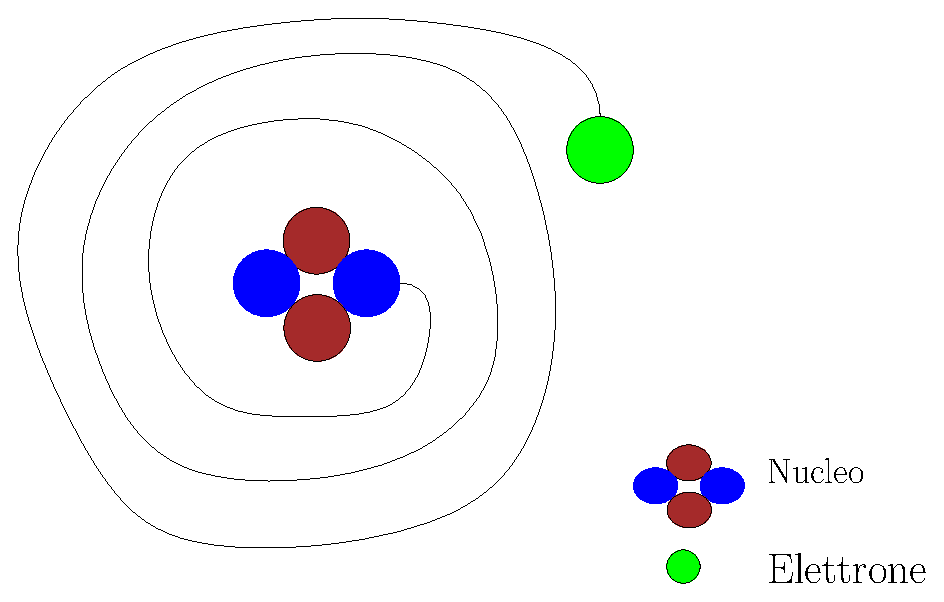
\includegraphics[width=5cm]{img/instmodRuth.eps}
  \caption[limModAtom]{Limiti del modello atomico di Rutherford}
  \label{fig:limModAtom}
\end{figure}
\clearpage
\section{Onda}
\label{sec:onde}
\begin{defi}
  Un’onda è una perturbazione che nasce da una sorgente e si propaga nel TEMPO e nello SPAZIO,
  trasportando ENERGIA.
  \begin{figure}[ht!]
    \centering
    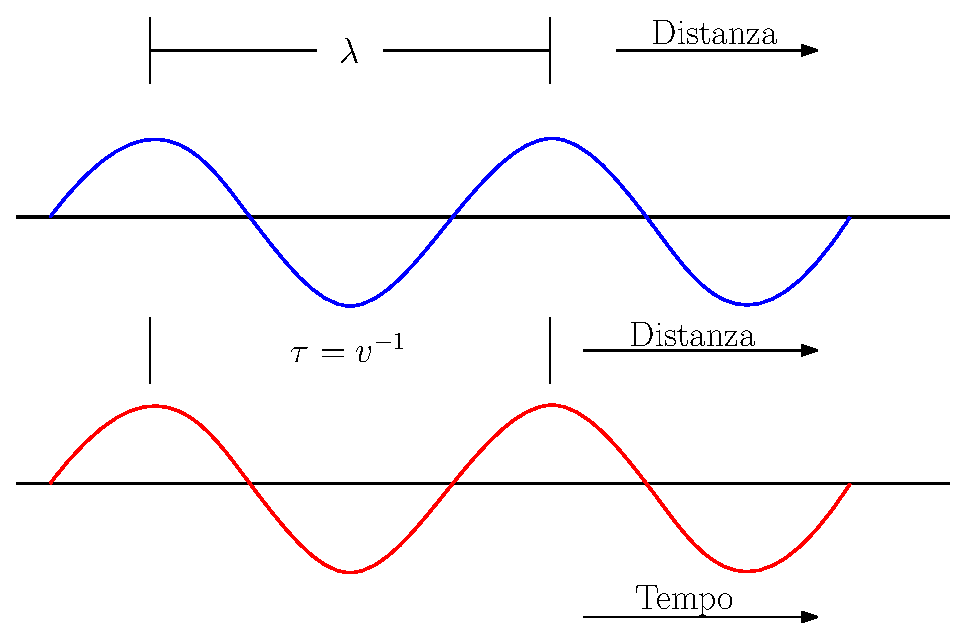
\includegraphics[width=6cm]{img/segnali.eps}
    \caption{Esempio onde}
    \label{fig:esonde}
  \end{figure}\\
  Il $\lambda$ è la distanza tra due massimi o due minimi successivi. 
\end{defi}

\subsection{Onde elettromagnetiche}
\label{sec:ondeElettro}

\begin{defi}
  Una radiazione elettromagnetica può essere considerata com un campo elettromagnetico oscillante che
  si propaga nello spazio. {\color{red}La luce è una radiazione elettromagnetica, e ha quindi una natura
    ondulatoria.}
\begin{figure}[th!]
    \centering
    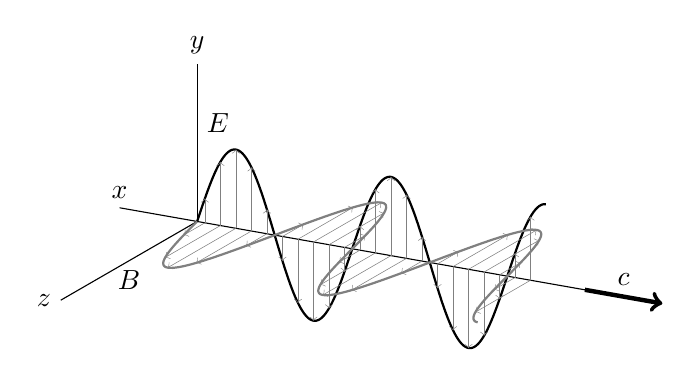
\begin{tikzpicture}[x={(-10:1cm)},y={(90:1cm)},z={(210:1cm)}]
    % Axes
    \draw (-1,0,0) node[above] {$x$} -- (5,0,0);
    \draw (0,0,0) -- (0,2,0) node[above] {$y$};
    \draw (0,0,0) -- (0,0,2) node[left] {$z$};
    % Propagation
    \draw[->,ultra thick] (5,0,0) -- node[above] {$c$} (6,0,0);
    % Waves
    \draw[thick] plot[domain=0:4.5,samples=200] (\x,{sin(deg(pi*\x))},0);
    \draw[gray,thick] plot[domain=0:4.5,samples=200] (\x,0,{sin(deg(pi*\x))});
    % Arrows
    \foreach \x in {0.1,0.3,...,4.4} {
      \draw[->,help lines] (\x,0,0) -- (\x,{sin(deg(pi*\x))},0);
      \draw[->,help lines] (\x,0,0) -- (\x,0,{sin(deg(pi*\x))});
    }
    % Labels
    \node[above right] at (0,1,0) {$E$};
    \node[below] at (0,0,1) {$B$};
\end{tikzpicture}
    \caption{Onde elettromagnetiche}
    \label{fig:ondelect}
\end{figure}
\begin{center}
  \begin{minipage}{.5\linewidth}
    \[
      c = \frac{E}{B}
    \]
    \begin{tabular}{r@{${}={}$}p{.8\linewidth}}
      $E$ & ampiezza del campo elettrico \\
      $B$ & ampiezza del campo magnetico (\texttt{valori istantanei}) \\
      $c$ & velocità della luce ($3\times10^8\mathrm{m/s}$) \\
    \end{tabular}
  \end{minipage}%
  \begin{minipage}{.5\linewidth}
    \[
      c = \frac{1}{\sqrt{\mu_0 \varepsilon_0}}
    \]
    \begin{tabular}{r@{${}={}$}p{.8\linewidth}}
      $\mu_0$ & permeabilità magnetica nel vuoto, $\mu_0 = 1.3\times10^{-6}\,\mathrm{N/A^2}$ \\
      $\varepsilon_0$ & permeabilità elettrica nel vuoto, $\varepsilon_0 = 8.9\times10^{-12}\,\mathrm{C^2/N m^2}$ \\
    \end{tabular}
  \end{minipage}
\end{center}
\end{defi}
\begin{nota}
  La luce consiste in un campo elettrico, un campo magnetico oscillanti e orientati perpendicolarmente
  tra loro, ma anche perpendicolarmente alla alla direzionedi propagazione del raggio.
\end{nota}

\subsection{Velocità di una radiazione elettromagnetica}
\label{sec:veldiunaradelect}

Nel vuoto una radiazione elettromagnetica si propaga alla velocità della luce\footnote{Essendo la luce
  stessa facente parte della suddetta catagoria}. La formula che va a definire tale aspetto è la seguente:
\begin{equation}
  \label{eq:veldiunaradelect}
  \lambda\cdot v=C
\end{equation}
Di cui:
\begin{description}
\item[$\lambda$ =] La lunghezza d'onda (km, m, cm, \ce{\mu m}, nm, Å)\footnote{\ce{\mu=10^{-6}m}; \ce{nm=10^{-9}m}, Å=\ce{10^{-10}m}}
\item[v =] La frequenza (cicli per sec = Hertz o Hz)
\item[C =] Una costante che nel vuoto è pari a $3.00\times 10^8 m/sec$
\end{description}
\clearpage
\begin{oss}
  Da questo possiamo dedurre che \ce{\lambda} e v risultano essere inversamente proporzionali, infatti,
  più aumenta una l'altra tende a diminuire.
\end{oss}
\begin{nota}
  Sul sito di Nikon è disponibile una dimostrazione per mostrare le proporzioni partendo da elettrone
  ad una galassia, il suo nome è Nikon universcale, è un sito ben fatto e richiede JS (JavaScrit)
  attivo nel proprio browser, per accedere alla dimostrazione clicca
  \href{https://www.nikon.com/company/corporate/sp/universcale/}{qui}\footnote{https://www.nikon.com/company/corporate/sp/universcale/}.
\end{nota}

\subsection{Effetto fotoelettrico}
\label{sec:effettofotoelettrico}

\begin{defi}
  L'effetto fotoelettrico è quel fenomeno che consiste nell'emissione, da parte di un metallo, di
  elettroni quando viene investito da radiazioni elettromagnetica avente una determinata energia.
  Chi scoprì questo particolare fenomeno fu il fisico tedesco Heinrich Rudolf Hertz.\\
  Gli elettroni espulsi nel fenomeno dell'effetto fotoelettrico sono normalmente trattenuti all'interno
  del metallo da una certa energia e per espellerla all'esterno, occorre, naturalmente, invstire il
  metallo con una radiazione elettromagnetica avente energia \ce{E=h.v} (in cui \ce{h} sta è la costante di Plank  almeno uguale ell'energina che vale $6.6262\cdot 10^{-34}J\cdot s$)
  li trattiene ``\ce{v=v0}''\footnote{In cui \ce{v0} è la frequenza critica, ed è caratteristica di
    ogni metallo}.
  \begin{description}
  \item[$v<v_0$] Una luce con una frequenza inferiore a \ce{v0}, anche se molto intensa non
    produrrà il suddetto fenomeno, perché la frequenza non è sufficientemente alta, quindi l'elettricità
    resterà intrappolata nel metallo.
  \item[$v>v_0$] Una luce di frequanza superiore a \ce{v0} avrà il seguente effetto, gli elettroni
    che vengono emessi mostreranno un energia cinetica tanto la differenza di frequenza tra \ce{v0} e
    v, più sarà grande maggiore sarà l'energia cinetica.
  \end{description}
  Per accedere al simulatore basta andare nel sito del \href{https://phet.colorado.edu/sims/cheerpj/photoelectric/latest/photoelectric.html?simulation=photoelectric&locale=it}{PhET}\footnote{https://phet.colorado.edu/sims/cheerpj/photoelectric/latest/photoelectric.html?simulation=photoelectric\&locale=it}, in
  cui potrete fare dei test cambiando il tipo di metallo, la frequenza e l'intensità della luce.
\end{defi}
\begin{nota}
  La scoperta dell'effetto fotoelettrico, influì nello sviluppo delle Teorie di Einstein a conferma
  delle sue ipotesi che la luce potesse manifestare oltre che una natura ondulatoria, anche una natura
  corpuscolare. Infatti, solo particelle cariche di sufficiente energia sarebbero in grado di spostare
  alre particelle (\texttt{elettroni del metallo}) e di cui impartire loro una accelerazione tanto
  maggiore quanto era la frequenza che delle luce impegnata.
\end{nota}
Ma cosa succede davvero quando $v<v_0$ e si aumenta l'intensità luminosa? La risposta è semplice,
in quel caso con l'aumento della intensità luminosa si va ad aumentare il numero dei fotoni incidenti
ma cianscuno di essi non ha l'energia sufficenter per estrarre gli elettroni.

\subsection{Spettri di emissione di atomi}
\label{sec:spemdiatom}

\begin{defi}
  Gli atomi \texttt{eccitati} emettono radiazioni solo di solo di certe lunghezze d'onda. La lunghezza d'onda
  della luce emessa varia al variare dall'elemento.
  \begin{figure}[ht!]
    \centering
    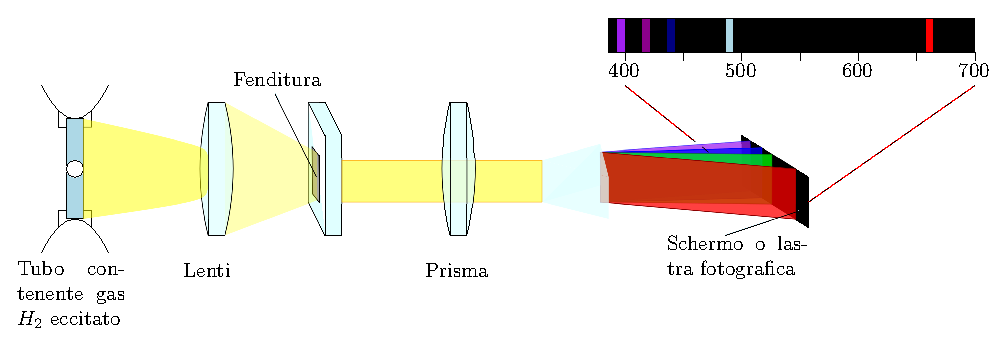
\includegraphics[width=14cm]{img/spettriColatom.eps}
    \caption{Spettri colori emessi dal \ce{H2}}
    \label{fig:h2spttricolor}
  \end{figure}
\end{defi}

\section{Spettri Atomici e Teoria di Bohr}
\label{sec:atomodiBohr}
\begin{defi}
  Gli spettri atomici a righe suggeriscono l'esistenza di livelli energetici definiti. Bohr (1885-1962) propose un modello atomico capace di interpretare con semplicità gli spettri atomici dell'idrogeno.
  \begin{figure*}[ht!]
    \centering  
    \bohr[2]{1}{He}
    \caption{Modello atomico di Bohr}
    \label{fig:Modatombohr}
  \end{figure*}

  L'atomo è costituito da un nucleo centrale e l'elettrone gli ruota attorno come un pianeta attorno
  al sole. L'\ce{e-} può occupare solo certe ORBITE chiamate STATI STAZIONARI, dove l'\ce{e-} si trova in STATI
  QUANTIZZATI DI ENERGIA.
  \begin{equation}
    \label{eq:energiastato}
    \text{Energia dello stato } = -\frac{R_H}{n^2}
  \end{equation}
  In cui:
  \begin{description}
  \item[\ce{R_H} =] $109677.581cm^{-1}$ (costante di Rydberg)
  \item[n =] 1,2,3,4,5,\dots NUMERO QUANTICO PRINCIPALE
  \end{description}
  Se gli \underline{elettroni} si trovano in stati energetici quantizzati, la transizione tra uno stato stazionario
  iniziale e quallo finale coinvolge quantità di energia. L'elettrone può passare dallo stato iniziale a quello
  finale {\color{blue}acquistando l'energia necessaria tramite l'assorbimento di un fotone o rilascandone per
    tornare ad un orbitale inferiore}\footnote{Sostanzialmente l'elettrone più energia avrà più sarà lontano al
    nucleo, meno energia avrà più starà vicino}.
  Per calcolare l'energia del fotone assorbito bisogna utilizzare la seguente formula:
  \begin{equation}
    \label{eq:energiafotoneassorbito}
    E_f-E_i=hv
  \end{equation}
  Di cui h è la Costante di Plank. 
\end{defi}
\begin{nota}
  La teoria, per la quale Bohr ricevette il Premio Nobel nel 1922, rappresenta la rottura con la fisica classica,
  introduce i concetti di numero quantico e stato stazionario ed è in grado di spiegare gli spettri dell’H.
\end{nota}
\begin{oss}
  La quantizzazione vene introdotta arbitrariamente; gli spettri degli atomi \textbf{non-idrogenoidi} non sono
  bene interpretati; posizione ed energia dell'elettrone vengono assegnati contemporaneamente; l'origine del legame
  chimico non viene spiegata. Da questo si può dedurre che il modello ipotizzato da Bohr è incompleto e non
  funzionale visto che butta in mezzo alcuni concetti che non sono validi per tutti gli elementi e quindi
  irrealistico.
\end{oss}

\section{Relazione di De Broglie}
\label{sec:deBroglie}
Nel 1924 De Broglie (1892-1987) avanzò l'ipotesi secondo la quale a ogni oggetto in movimento può essere associata
una lunghezza d'onda, secondo l'equazione:
\begin{eqnarray}
  \label{eq:deBroglie}
  \lambda = \frac{h}{mv} & v=\text{Velocità dell'oggetto}
\end{eqnarray}
Per qun oggetto macroscopitco la lunghezza  d'onda associata è talmente piccola da non permettere di mettere in
evidenzia le proprietà ondulatorie dell'oggetto.\\
Ora, affronteremo due esercizi per comprendere meglio questo concetto che altrimenti potrebbe non essere molto
chiaro.
\begin{ess}
  Prendiamo un pallona da calcio che a una massa (m) di 0.5kg e una velocità (v) di $30\nicefrac{m}{s}$ se andiamo a
  calcolare la lunghezza d'onda otterremo il seguente risultato:
  \begin{eqnarray*}
    \lambda=\frac{h}{mv} = \frac{6.62\times 10^{-34}Js}{0.5kg\times 30m s^{-1}}=\frac{6.62\times 10^{-34}kgm^2s^2s}{0.5kg\times 30m s^{-1}}=4.4\times 10^{-35}m
  \end{eqnarray*}
  quindi il risultato finale è che la lunghezza d'onda è pari a $4.4\times 10^{-35}$m
\end{ess}
Mentre, se andiamo a prendere un esempio microscopico il risultato è il seguente:
\begin{ess}
  Prendiamo un elettrone di massa (m) di $9\times 10^{-31}kg$ e una velocità di $2\times 10^{6}m/s$ se andiamo a
  calcolare la lunghezza d'onda otterremo il seguente risultato:
  \begin{eqnarray*}
    \lambda = \frac{h}{mv} = \frac{6.62\times 10^{-34}Js}{9\times 10^{-31}kg\times 2\times 10^{6}m/s}=\frac{6.62\times 10^{-34}kgm^2s^2s}{9\times 10^{-31}kg\times 2\times 10^{6}m/s}=3.68\times 10^{-10}m
  \end{eqnarray*}
  quindi il risultato finale è che la lunghezza d'onda è pari a $3.68\times 10^{-10}m$
\end{ess}

\subsection{Dualismo Onda-particella}
\label{sec:dualismoOnda-part}
\begin{defi}
  In fisica, per dualismo onda-particella si definisce la duplice natura, sia corpuscolare sia ondulatoria, del
  comportamento della materia e delle radiazione elettromagnetica. Quest'idea nella fisica dei quanti inizia nel
  1900 con lo studio dello spettro della radiazione di compo nero di Plank da cui si ricaverà la costante omonima
  $h=6.62\times 10^{-34}$, per poi essere succeduto degli studi di Einstein (1905-1909) da cui si otterrà la formula
  per ricavare l'energia $E=hv$ e nello studio sul dualismo onda-particella anche la variazione $\sigma^2(\bar{n})$
  che mostrava due termini, una lineare e uno quadratico\footnote{Quadratico = un numero elevato 2} un $\bar{n}$,
  numero medio di quanti d'energia a frequanza $v$ da attribuire a ciascun risonatore responsabile dell'emissione
  o assorbimento dei radiazione.
  \begin{equation}
    \label{eq:numeromediodiquanti}
    \sigma^2(\bar{n})=\bar{n}+\bar{n}^2
  \end{equation}
  Questa caratteristica apparve subito sconcertante perch era noto che i sistemi di particelle hanno una dipendeza
  lineare in $\bar{n}$ della varianza:
  \begin{equation}
    \label{eq:rapportodipendenteadn}
    \sigma^2(\bar{n})=\bar{n}
  \end{equation}
  mentre quelli formati da onde mostrano una dipendenza quadratica:
  \begin{equation}
    \label{eq:ondedipendenzaquadratica}
    \sigma^2(\bar{n})=\bar{n}^2
  \end{equation}
  Poi nel 1924 troviamo la Relazione di De Broglie (\ref{sec:deBroglie}).
\end{defi}

\section{Principio di Indeterminazone di Heisenberg}
\label{sec:heisenberg}
\begin{defi}
  Il dualismo onda-materia si manifesta a livello microscopico:
  \begin{equation}
    \label{eq:dualismoondamateria}
    \Delta x \cdot \Delta (m\cdot v)\geq \frac{h}{4\pi}
  \end{equation}
  Di cui $\Delta$ indica l'errore (l'incertezza) della misura.
\end{defi}
\begin{prin}
  ``La posizione ed il momento \ce{(m.v)} di un elettrone non possono essere misurati {\color{red}simultaneamente}
  con assoluta accuratezza''
  \begin{enumerate}
  \item È una conseguenza della natura ondulatoria delle particelle microscopiche.
  \item Non è possibile descrivere un'orbita dell'elettrone intorno al nucleo.
  \end{enumerate}
\end{prin}
Anche in questo caso situazione sarà più chiara se andiamo a svolgere due esercizi prendendo un oggetto macroscopitco
e uno microscopico.
\begin{ess}
  Prendiamo un a sferetta di pari a $m=10^{-3}$ e di $g=10^{-6}kg$:
  \begin{equation*}
    \Delta x \Delta v_x \cong \frac{6.62\times 10^{-34}J\cdot s}{10^{-6}kg}\cong 6.62\times 10^{-28}m^2/s
  \end{equation*}
  si prenda $\Delta x = 10^{-12}m$, risulta $\Delta v_x= 6.62\times 10^{-16}m/s$
\end{ess}
\begin{ess}
  Prendiamo un elettrone con un $m=10^{-27}$ e un g di $10^{-30}kg$
  \begin{equation*}
    \Delta x \Delta v_x\cong \frac{6.62\times 10^{-34}J\cdot s}{10^{-30}kg}\cong 6.62\times 10^{-4}m^2/s
  \end{equation*}
  si prende $\Delta x = 10^{-12}m$, risulta $\Delta v_x= 6.62\times 10^8m/s$
\end{ess}

\section{Equazione d'onda (1926)}
\label{sec:equazionedonda}
\begin{defi}
  L'equazione d'onda:
  \begin{equation*}
    \frac{\hbar^2}{2m}\nabla^2\psi_n+(E-V) \psi_n=0
  \end{equation*}
  proposta da Schroedinger per descrivere il comportamento di un elettrone sottoposto all'azione del nucleo si basa
  sul:
  \begin{description}
  \item[1)] carattere ondulatorio dell'elettrone
  \item[2)] carattere probabilistico della conoscenza
  \item[\ce{\psi} =] funziona d'onda deve essere \textbf{continua}, da un \textbf{solo valore, finita}.
  \end{description}
  Funzione soluzione dell'equazione d'onda, che permette di calcolare l'Energia
  \begin{itemize}
  \item È funzione della distanza e di due angoli.
  \item Ad ogni orbitale, caratterizzato da tre \textbf{numeri quantici n, l, m,} corrisponde un valore di energia
  \item come ogni funzione d'onda l'orbitale presenta nodi subisce conseguente combiamento di fase
  \item \textbf{NON} descrive la posizione esatta dell'elettrone
  \item \textbf{Il significato fisico è legato a \ce{\Psi2}} che è \textbf{proporzionale alla probabilità} di trovare
    un elettrone in un determinato punbto.
  \end{itemize}
\end{defi}

\section{I numeri quantici}
\label{sec:numQuant}

\begin{table}[ht!]
  \centering
  \begin{tabular}{lll}
    Simbolo&Valore&Descrizione\\\hline
    n (principale) & 1,2,3,\dots & Dimensione orbitale ed energia \ce{E=-C/n^2} (Guscio)\\\hline
    l (angolare)   & 0,1,2,\dots,n-1 & Forma orbitale o tipo (Sottoguscio)\\\hline
    \ce{m_l} (magnetico)& -l,0,+l & Orientazione orbitale\\\hline
  \end{tabular}
  \caption{Numeri quantici}
  \label{tab:numquant}
\end{table}
Nel caso di $l$ corrisponde al numero di orbitali nel sottoguscio = 2l+1

\subsection{Ralazioni tra numeri quantici}
\label{sec:relnumquant}

\begin{table}[ht!]
  \centering
  \begin{tabular}{cccccc}
    \multicolumn{2}{c}{Numeri quantici} & &Nome comune dell'orbitale & \multicolumn{2}{c}{Numero totale di orbitali}\\\hline 
    \ce{n}&\ce{l}& \ce{m_l} & \\\hline
    1 & 0 & 0 & 1s & 1 & 1\\\hline
    \multirow{2}{*}{2} &0&0&2s&1&\multirow{2}{*}{4} \\
                                        &1&-1,0,+1&2p&3& \\\hline
                                        \multirow{3}{*}{3}&0&0&3s&1 &\multirow{3}{*}{9} \\
                                        &1&-1,0,+1&3p&3& \\
                                        &2&-2,-1,0,+1,+2&3d&5& \\\hline
                                        \multirow{4}{*}{4}&0&0&4s&1&\multirow{4}{*}{16} \\
                                        &1&-1,0,+1&4p&3& \\
                                        &2&-2,-1,0,+1,+2,+3&4d&5& \\
                                        &3&-3,-2,-1,0,+1,+2,+3&4f&7&\\\hline
  \end{tabular}
  \caption{Relazione tra numeri quantici}
  \label{tab:relnumquant}
\end{table}
\clearpage
\subsection{Rappresentazione grafica degli orbitali atomici}
\label{sec:orbatom}
Facendo una descrizione approssimativa a palloncini: si racchiude con una superficie limite uno spazio
contenente il $90\%$ di probabilità di trovarvi l'elettrone e si indica il segno della funzione
originaria. Prendono il nome dal valore di l.
\begin{figure}[ht!]
  \centering
  
\begin{tikzpicture}
 \orbital[pos = {(2,5.5)}]{lobe}
 \node[above] at (2.5,6) {simple lobe};

 \orbital[pos = {(0,5.5)}]{s}
 \node[above] at (0,6) {s};

 \orbital[pos = {(0,3)}]{px}
 \node[above] at (0,4) {p$_x$};
 \orbital[pos = {(2,3)}]{py}
\node[above] at (2,4) {p$_y$};
\orbital[pos = {(4,3)}]{pz}
 \node[above] at (4,4) {p$_z$};

 \orbital[pos = {(0,0)}]{-px}
 \node[above] at (0,1) {-p$_x$};
 \orbital[pos = {(2,0)}]{-py}
 \node[above] at (2,1) {-p$_y$};
 \orbital[pos = {(4,0)}]{-pz}
 \node[above] at (4,1) {-p$_z$};

 \orbital[pos = {(0,-3)}]{dxy}
 \node[above] at (0,-2) {d$_{xy}$};
 \orbital[pos = {(2,-3)}]{dxz}
 \node[above] at (2,-2) {d$_{xz}$};
 \orbital[pos = {(4,-3)}]{dyz}
 \node[above] at (4,-2) {d$_{yz}$};

 \orbital[pos = {(0,-5)}]{dx2y2}
 \node[below] at (0,-6) {d$_{x^2-y^2}$};
 \orbital[pos = {(2,-5)}]{dz2}
 \node[below] at (2,-6) {d$_{z^2}$};
\end{tikzpicture}
  \caption{Rappresentazione grafica degli orbitali atomici}
  \label{fig:rapgrorat}
\end{figure}
